\documentclass[conference]{IEEEtran}

\usepackage{cite}
\usepackage{amsmath}
\usepackage{amssymb}
\usepackage{graphicx}
\usepackage{booktabs}
\usepackage{microtype}
\usepackage{url}
\usepackage{textcomp}
\usepackage[hidelinks]{hyperref}

\newcommand{\FV}{figures}
\makeatletter\newcommand{\tabin}[1]{\@@input #1 }\makeatother

\begin{document}

\title{Multi-Label Retinal Disease Detection on RFMiD under Three Label Taxonomies:\\DINOv2 ViT-L with a Residual Attention Token Head, Retinal Initialisation, BFPC-Net Baselines and Small Ensembles}

\author{\IEEEauthorblockN{Xabat Arin}
\IEEEauthorblockA{\texttt{xabatarin01@gmail.com}}}

\maketitle

\begin{abstract}
A fundus photograph often shows more than one abnormality, so a screening model should give an independent decision for each condition.
We study multi-label classification on the Retinal Fundus Multi-Disease Image Dataset (RFMiD) under three label taxonomies built from the same 45 RFMiD columns: an ODIR-style seven-label scheme (ODIR-7), a ten-cluster scheme obtained by clustering supervised image embeddings (Cluster-C), and a fourteen-label scheme with twelve supervised latent groups, a rare-disease group and a healthy label (Sup-K12).
The main model is a DINOv2 ViT-L/14 backbone, partially fine-tuned (last four blocks), with a residual attention token head (ViT-RA). We compare it with a plain DINOv2 head, with initialisation from a retinal foundation model (RETFound-DINOv2), with $392$ versus $518$\,px inputs, with BFPC-Net-style ResNet-50 baselines, and on Sup-K12 with Inception-v3 and with focal versus asymmetric losses.
Per-label thresholds are fitted on validation data only, either to maximise $F_2$ or to reach a recall of at least 0.8.
All 38 single models and 2--3-member equal-weight ensembles are evaluated on the official 640-image test set, with 2000-resample bootstrap confidence intervals (CIs) and paired bootstrap differences.
Ensembles selected on validation reach a test macro $F_2$ of 0.835 [0.817, 0.852] and a macro AUROC of 0.954 on ODIR-7, 0.775 [0.745, 0.803] and 0.940 on Cluster-C, and 0.687 [0.636, 0.732] and 0.937 on Sup-K12.
The ensemble is significantly better than the validation-selected single model on ODIR-7 ($\Delta F_2=+0.023$ [+0.008, +0.039]) and Sup-K12 (+0.061 [+0.012, +0.111]), but not on Cluster-C (+0.002 [$-$0.016, +0.021]).
Retinal initialisation did not improve over DINOv2 initialisation in any paired comparison. Higher resolution helped only on Cluster-C.
Grad-CAM maps are qualitative only. The models are research prototypes, not medical devices.
\end{abstract}

\begin{IEEEkeywords}
retinal fundus, multi-label classification, vision transformer, DINOv2, RETFound, label taxonomy, ensembles, bootstrap, Grad-CAM
\end{IEEEkeywords}

\section{Introduction}
Retinal fundus photography is a low-cost, non-invasive way to examine the posterior segment of the eye, and deep learning has shown strong results for individual diseases such as diabetic retinopathy~\cite{gulshan2016dr}.
In practice, however, a fundus image may show several abnormalities at once, and a screening tool should flag any of them rather than answer a single binary question.
This motivates a multi-label formulation, in which each image receives an independent decision for each condition.

Three difficulties make this setting hard.
First, the label distribution is imbalanced: RFMiD~\cite{pachade2021rfmid} has 45 disease columns, many with only a handful of positives, so some grouping is unavoidable. The way the columns are grouped (the \emph{taxonomy}) changes both the task and the numbers that can be reported.
Second, large transformer backbones are expensive to fine-tune and easy to overfit on a dataset of a few thousand images.
Self-supervised vision transformers such as DINOv2~\cite{oquab2024dinov2} provide strong general-purpose features, and retinal foundation models such as RETFound~\cite{zhou2023retfound} promise domain-specific ones. It is not obvious which initialisation, input resolution and head work best.
Third, the evaluation is fragile. With 640 test images and labels that have tens of positives, differences of 0.01--0.02 in a macro metric are often within sampling noise.

This paper extends our earlier single-model study (a ten-label DINOv2 ViT-L/14 classifier with a macro test AUROC of 0.904) to a controlled comparison across three taxonomies, two backbone families, two initialisations, two resolutions and small ensembles.
The contributions are:
\begin{itemize}
  \item three reproducible RFMiD label taxonomies (ODIR-7, Cluster-C, Sup-K12), with explicit column-to-label maps and per-split positive counts;
  \item a DINOv2 ViT-L/14 with a residual attention token head (ViT-RA), and a comparison with a plain DINOv2 head, RETFound-DINOv2 initialisation, $518$\,px inputs and BFPC-Net-style ResNet-50 baselines~\cite{li2022bfpc};
  \item an evaluation protocol that fits every threshold and every selection (model, ensemble) on validation data only and reports test metrics with 2000-resample bootstrap CIs and paired differences;
  \item ablations, seed-variance estimates, per-class results, ROC/PR curves and a qualitative Grad-CAM comparison, together with an explicit list of what could not be verified.
\end{itemize}

\section{Related Work}
\textbf{Retinal disease datasets.}
RFMiD~\cite{pachade2021rfmid} provides 3200 fundus images with 45 disease annotations plus a \texttt{Disease\_Risk} flag, and official training, validation and test splits, which we use unchanged.
ODIR-2019~\cite{odir2019} groups patient-level diagnoses into eight categories (normal, diabetes, glaucoma, cataract, AMD, hypertension, myopia, other). Our ODIR-7 taxonomy maps RFMiD columns onto this scheme.
Earlier large-scale work on diabetic retinopathy detection~\cite{gulshan2016dr} focused on a single condition.

\textbf{Multi-label fundus architectures.}
BFPC-Net~\cite{li2022bfpc} combines an image augmentation module, a ResNet-50~\cite{he2016resnet} with residual attention, and a feature-fusion module that merges the left and right eyes of a patient, and reports very high scores on ODIR.
RFMiD has no left/right pairing, so we use a single-image variant and a ``dual-view'' variant that fuses two augmented views of the same image.
Inception-v3~\cite{szegedy2016inception} is a widely used CNN baseline for fundus classification.

\textbf{Vision transformers and foundation models.}
The Vision Transformer (ViT)~\cite{dosovitskiy2021vit} splits an image into patches and processes them with transformer blocks.
DINOv2~\cite{oquab2024dinov2} trains ViTs with self-supervision on a curated image collection and yields features that transfer well without task-specific supervision.
RETFound~\cite{zhou2023retfound} is a foundation model pre-trained on large collections of retinal images; we use its DINOv2-based release as an alternative initialisation.
FLAIR~\cite{silva2025flair} is a language-image retinal model trained on many public fundus datasets; we use its ResNet-50 vision encoder to initialise one BFPC baseline.

\textbf{Partial fine-tuning.}
Gradually adapting only the upper layers of a pre-trained network, as in gradual unfreezing~\cite{howard2018ulmfit}, reduces the number of trainable parameters and the risk of forgetting pre-trained features.
We follow this idea by unfreezing the last transformer blocks with a separate, smaller learning rate than the head.

\textbf{Imbalance and optimisation.}
Weighting positive examples in the binary cross-entropy is a standard way to counter label imbalance. Focal loss~\cite{lin2017focal} down-weights easy examples, and the asymmetric loss (ASL)~\cite{ridnik2021asl} treats positives and negatives differently and discards easy negatives, which suits multi-label tasks with many negatives.
Models are optimised with AdamW~\cite{loshchilov2019adamw}, a variant of Adam~\cite{kingma2015adam} with decoupled weight decay, and a cosine learning-rate schedule~\cite{loshchilov2017sgdr}.
For imbalanced problems, precision--recall analysis is generally more informative than ROC analysis alone~\cite{saito2015prroc}, so we report both.
Uncertainty in the test estimates is quantified with the bootstrap~\cite{efron1993bootstrap}.

\textbf{Explainability.}
Grad-CAM~\cite{selvaraju2017gradcam} produces class-specific localisation maps from gradients; we use an adaptation to ViT patch tokens (Section~\ref{sec:gradcam}).
Monte Carlo dropout~\cite{gal2016dropout} is a common way to estimate predictive uncertainty but was not evaluated here.

\section{Methodology}
\subsection{Data and label taxonomies}
We use the official RFMiD splits: 1920 training, 640 validation and 640 test images.
The 45 disease columns are mapped to labels by a logical OR of their columns. The three taxonomies are:

\textbf{ODIR-7} (7 labels): N, D, G, C, A, M, O, following the ODIR scheme as adopted by BFPC-Net~\cite{li2022bfpc}. N is defined by \texttt{Disease\_Risk}\,=\,0. ODIR's hypertension class is dropped because RFMiD has no hypertension column. ``C'' is a \emph{media-opacity proxy} (MH, AH, VH), not true cataract, and ``G'' is an optic-disc proxy (ODC, ODP, ODE, AION).

\textbf{Cluster-C} (10 labels): pathology columns are embedded with a supervised ResNet-50 multi-label encoder, reduced with PCA to 32 dimensions and clustered with $k$-means ($k=10$, silhouette 0.263). Each column is assigned to a cluster. This taxonomy has no healthy label.

\textbf{Sup-K12} (14 labels): twelve groups from a supervised latent regrouping ($k=12$), a group ``otros'' for 21 rare columns (fewer than 10 training positives), and a healthy label ``sano'' (\texttt{Disease\_Risk}\,=\,0 and no active disease column). Metrics on Sup-K12 are computed over the 13 disease labels; ``sano'' is excluded from the macro averages.

\autoref{tab:labels} lists the labels and the number of positive images per split.
Several Sup-K12 groups have very few test positives (g03\_pt: 4, g05\_ms: 7, g09: 14), so their per-class metrics are unreliable.
The dataset files carry no patient identifier, so overlap of patients across splits cannot be checked.

\begin{table}[t]
\centering
\caption{Labels and number of positive images per split (Train/Val/Test). Column lists are RFMiD abbreviations.}
\label{tab:labels}
\scriptsize
\setlength{\tabcolsep}{2.5pt}
\begin{tabular}{@{}lp{3.6cm}rrr@{}}
\toprule
Label & RFMiD columns & Tr & Va & Te \\
\midrule
\multicolumn{5}{@{}l}{\textit{ODIR-7}}\\
N & \texttt{Disease\_Risk}=0 & 401 & 134 & 134 \\
D & DR, EDN, CWS & 392 & 139 & 130 \\
G & ODC, ODP, ODE, AION & 420 & 123 & 135 \\
C & MH, AH, VH & 333 & 106 & 109 \\
A & ARMD, DN & 234 & 83 & 76 \\
M & MYA, TSLN, TD & 289 & 100 & 86 \\
O & all remaining columns (30) & 376 & 125 & 122 \\
\midrule
\multicolumn{5}{@{}l}{\textit{Cluster-C}}\\
ARMD\_TSLN & ARMD, TSLN & 255 & 97 & 80 \\
DR & DR & 376 & 132 & 124 \\
BRVO\_CRVO & BRVO, CRVO & 101 & 31 & 32 \\
MYA & MYA & 101 & 34 & 32 \\
DN & DN & 138 & 46 & 46 \\
LS\_TV\_AH & LS, TV, AH, RT & 79 & 27 & 27 \\
ERM\_MS\_CSR & ERM, MS, CSR, ODP, EDN, \dots\ (27) & 242 & 94 & 89 \\
ODC\_CWS & ODC, CWS & 284 & 75 & 93 \\
ODE\_AION\_RS & ODE, AION, RS, CRAO & 119 & 42 & 35 \\
MH & MH & 317 & 102 & 104 \\
\midrule
\multicolumn{5}{@{}l}{\textit{Sup-K12}}\\
g01 & AION, ODE & 75 & 26 & 21 \\
g02 & CSR, DN, MHL, RPEC & 202 & 65 & 66 \\
g03 & PT & 11 & 2 & 4 \\
g04 & ERM, ODP & 77 & 33 & 29 \\
g05 & MS & 15 & 5 & 7 \\
g06 & CRS, RS & 75 & 25 & 25 \\
g07 & BRVO, CRVO & 101 & 31 & 32 \\
g08 & DR, LS & 382 & 142 & 129 \\
g09 & AH, EDN, RT & 45 & 15 & 14 \\
g10 & ARMD, MYA, TSLN & 332 & 119 & 108 \\
g11 & MH & 317 & 102 & 104 \\
g12 & ODC & 282 & 72 & 91 \\
g13 otros & 21 rare columns & 49 & 29 & 21 \\
sano & healthy (not in macro) & 401 & 134 & 134 \\
\bottomrule
\end{tabular}
\end{table}

\subsection{Preprocessing and augmentation}
Images are resized to the model resolution ($392$ or $518$\,px for ViT-L/14, $448$\,px for Inception, $256$\,px for BFPC) and normalised with ImageNet statistics.
Training augmentation consists of random flips, small rotations, and colour and brightness jitter. BFPC models additionally use the image augmentation module of BFPC-Net~\cite{li2022bfpc}.
Some Sup-K12 models were evaluated with test-time augmentation (TTA: the average over flipped views) and without it (no-TTA); both are reported as separate entries.

\subsection{Models}
\textbf{ViT-RA (main model).}
A DINOv2 ViT-L/14~\cite{oquab2024dinov2,wightman2019timm} (304\,M parameters) whose last four transformer blocks and final normalisation are unfrozen.
The \emph{residual attention token head} works on the final patch tokens $T\in\mathbb{R}^{N\times d}$ and the class token $c$.
A channel gate $g_c=\sigma(\mathrm{MLP}(\mathrm{avg}(T))+\mathrm{MLP}(\max(T)))$ re-weights the feature channels.
A spatial gate (a linear map of the per-token mean and max over channels) gives a score to each token, and the softmax over these scores pools the tokens into a local descriptor $\ell$.
The output $\mathrm{LN}(c+\ell)$ (a residual global--local fusion) goes through dropout (0.2) and a linear classifier.

\textbf{ViT-D (plain DINOv2 head).} The same backbone and fine-tuning recipe with a linear head on the class token.

\textbf{Initialisation.} ``v2'' models start from the DINOv2 ViT-L/14 weights. ``fundus'' models start from RETFound-DINOv2~\cite{zhou2023retfound}, a retinal foundation model with the same architecture.

\textbf{BFPC baselines.} A ResNet-50 with residual attention and feature fusion in the style of BFPC-Net~\cite{li2022bfpc}, in a single-image variant and a dual-view variant that fuses two augmented views of the same image (RFMiD has no left/right pairs). One Sup-K12 BFPC baseline (\texttt{bfpc focal full}) was trained with focal loss.

\textbf{Sup-K12 models.} Inception-v3 at $448$\,px and ViT-D at $518$\,px, trained with ASL~\cite{ridnik2021asl} or focal loss~\cite{lin2017focal}, over three seeds (default, 1, 2). There are also earlier full-resolution baselines (\texttt{*\_focal\_full}) and a ViT-D initialised from RETFound (\texttt{asl fundus}).

\subsection{Training}
ViT models are trained for up to 80 epochs (patience 15) with AdamW~\cite{loshchilov2019adamw}, weight decay $10^{-4}$, head learning rate $10^{-3}$, backbone learning rate $10^{-5}$, a cosine schedule~\cite{loshchilov2017sgdr} with two warm-up epochs, mixed precision, gradient clipping at 1.0 and gradient checkpointing~\cite{chen2016checkpointing}. The batch size is 8 at $392$\,px and 4 at $518$\,px.
BFPC models are trained for up to 60 epochs with batch 16 at $256$\,px and label smoothing 0.1.
For ODIR-7 and Cluster-C the loss is a weighted binary cross-entropy with per-label positive weight
\begin{equation}
w_c=\min\!\left(\max\!\left(N_c^-/N_c^+,\,1\right),\,20\right),
\end{equation}
where $N_c^+$ and $N_c^-$ are the training positives and negatives of label $c$.
The checkpoint with the lowest validation loss is kept.
All models are implemented in PyTorch~\cite{paszke2019pytorch} and trained on Kaggle or Colab GPUs.

\subsection{Decision thresholds}
Each label gets its own threshold $t_c$, fitted on the \emph{validation} predictions only and then applied unchanged to the test set. There are two operating points:
\begin{itemize}
\item \textbf{F2-opt:} $t_c$ maximises the per-label $F_2$ on a grid $\{0.01,\dots,0.99\}$, which weights recall four times more than precision;
\item \textbf{R$\geq$0.8 (recall floor):} $t_c$ is the score of the $\lceil 0.8\,N_c^+\rceil$-th highest-scoring validation positive, so that validation recall is at least 0.8.
\end{itemize}

\subsection{Ensembles and model selection}
For each taxonomy we take the six single models with the highest validation macro $F_2$ and form every equal-weight average of two or three of them.
The final single model and the final ensemble are the ones with the highest \emph{validation} macro $F_2$; test results never enter selection.
We also report the single model with the best test score, for reference only.

\subsection{Metrics and statistics}
Per label we compute recall $R_c$, precision $P_c$, AUROC and average precision (AP). Macro recall and precision are the means over labels, and
\begin{equation}
F_2 = \frac{5\,\bar P\,\bar R}{4\,\bar P+\bar R},
\end{equation}
computed from the macro precision $\bar P$ and macro recall $\bar R$. We also report the macro F1 (the mean of per-label F1), the macro AUROC and the mean AP (mAP).
CIs are percentile intervals from 2000 bootstrap resamples of the 640 test images~\cite{efron1993bootstrap}. Thresholds are kept fixed.
Paired differences between two models reuse the \emph{same} resamples. A difference is called significant when its 95\% CI excludes zero.

\subsection{Grad-CAM}\label{sec:gradcam}
For ViT models we apply Grad-CAM~\cite{selvaraju2017gradcam} to the patch tokens at the output of \texttt{norm1} of the last block: the token activations are weighted by the mean gradient of the class logit, and a ReLU is applied.
For the Sup-K12 class-token head, the patch gradients at the block output are zero, so the same \texttt{norm1} hook is used.
Seven test images were chosen, one per ODIR-7 label (the most confident true positive of the ODIR-7 single model, preferring single-label images). For each image the map is computed for the most probable non-healthy class.

\section{Experimental Setup}
In total we evaluated 38 distinct single models (10 on ODIR-7, 9 on Cluster-C, 19 on Sup-K12) and 125 ensembles. The predictions of each model on validation and test were stored as arrays. Duplicate prediction files (identical test probabilities) were removed.
All evaluation scripts recompute every metric from these stored predictions. The ablation differences in \autoref{tab:ablation} were recomputed independently and reproduce the stored point estimates exactly.
The main evaluation scripts are in \texttt{results/final\_comparison\_20261030/scripts}. The figures and tables of this paper are generated by \texttt{paper/figures\_v3\_20261102/05\_paper\_v3\_figs\_tables.py}.

\section{Results}
\subsection{Headline results}
\autoref{tab:headline} shows the validation-selected single model and ensemble for each taxonomy at both operating points.
At the F2-opt point the ensembles reach a macro recall of 0.913 (ODIR-7), 0.809 (Cluster-C) and 0.750 (Sup-K12), with macro precisions of 0.62, 0.66 and 0.51.
The R$\geq$0.8 rule gives test recalls of 0.78--0.80 on ODIR-7 and Cluster-C, close to the target fixed on validation, and higher precision; on Sup-K12 the test recall falls to 0.68--0.70, which shows that the validation-fitted thresholds transfer less well when labels have few positives.
The macro AUROC does not depend on the thresholds and is 0.954, 0.940 and 0.937 for the three ensembles.

\begin{table*}[t]
\centering
\caption{Validation-selected single model and ensemble per taxonomy, test set (640 images), with 95\% bootstrap CIs. Thresholds and selection use validation only. Single models: ViT-RA 518 (ODIR-7), ViT-RA 518 (Cluster-C), ViT-D 518 focal seed 2 TTA (Sup-K12). Ensembles: ViT-RA 518 + ViT-RA 392 + ViT-RA fundus (ODIR-7); ViT-RA 518 + ViT-RA fundus (Cluster-C); ViT-D 518 focal seed 2 + Inception ASL + Inception ASL seed 1, all no-TTA (Sup-K12).}
\label{tab:headline}
\small
\begin{tabular}{@{}lllcccc@{}}
\toprule
Taxonomy & Model & Op. point & Macro recall & Macro prec. & Macro $F_2$ & Macro AUROC \\
\midrule
\tabin{\FV/tab_headline.tex}
\bottomrule
\end{tabular}
\end{table*}

\subsection{All single models}
Tables~\ref{tab:singles_odir}--\ref{tab:singles_sup} list every single model at the F2-opt point, ordered by test $F_2$, and \autoref{fig:forest} shows their CIs.
On ODIR-7 and Cluster-C the ViT-RA models with DINOv2 initialisation are at the top. On ODIR-7 the best test $F_2$ is 0.814 [0.794, 0.831] (ViT-RA 392) and the validation-selected ViT-RA 518 reaches 0.812; their CIs overlap almost completely.
BFPC is the weakest family on both taxonomies (0.770 and 0.708).
On Sup-K12 the best single models are the Inception-v3 ASL models (0.681 with TTA). The earlier \texttt{focal full} baselines are far behind (0.53--0.57).
The validation-selected Sup-K12 single model (ViT-D focal seed 2 TTA, validation $F_2$ 0.735) is only ninth on test (0.625). This gap between validation and test ranking is the clearest example of selection noise in this study.

\begin{table*}[t]
\centering
\caption{ODIR-7, single models, F2-opt thresholds. Test metrics with 95\% bootstrap CIs. RA: residual attention head; D: plain DINOv2 head; ``fundus'': RETFound-DINOv2 initialisation; 518: $518$\,px input (otherwise $392$).}
\label{tab:singles_odir}
\footnotesize
\begin{tabular}{@{}lcccccc@{}}
\toprule
Model & Val $F_2$ & Recall & Prec. & Test $F_2$ [95\% CI] & AUROC [95\% CI] & mAP \\
\midrule
\tabin{\FV/tab_singles_odir7.tex}
\bottomrule
\end{tabular}
\end{table*}

\begin{table*}[t]
\centering
\caption{Cluster-C, single models, F2-opt thresholds (same notation as \autoref{tab:singles_odir}).}
\label{tab:singles_cc}
\footnotesize
\begin{tabular}{@{}lcccccc@{}}
\toprule
Model & Val $F_2$ & Recall & Prec. & Test $F_2$ [95\% CI] & AUROC [95\% CI] & mAP \\
\midrule
\tabin{\FV/tab_singles_cluster_c.tex}
\bottomrule
\end{tabular}
\end{table*}

\begin{table*}[t]
\centering
\caption{Sup-K12, single models, F2-opt thresholds, 13 disease labels (``sano'' excluded). ``448''/``518'': input size; ASL: asymmetric loss; seed1/seed2: additional seeds; tta/notta: with or without test-time augmentation; ``focal full'': earlier baselines.}
\label{tab:singles_sup}
\footnotesize
\begin{tabular}{@{}lcccccc@{}}
\toprule
Model & Val $F_2$ & Recall & Prec. & Test $F_2$ [95\% CI] & AUROC [95\% CI] & mAP \\
\midrule
\tabin{\FV/tab_singles_sup_k12.tex}
\bottomrule
\end{tabular}
\end{table*}

\begin{figure*}[t]
\centering
\includegraphics[width=\textwidth]{\FV/fig_forest_f2.pdf}
\caption{Test macro $F_2$ (F2-opt thresholds) with 95\% bootstrap CIs for every single model and the validation-selected ensemble (red). Blue: ViT; purple: BFPC; grey: Inception.}
\label{fig:forest}
\end{figure*}

\subsection{Ensembles}
\autoref{tab:ens} lists the four ensembles with the highest validation $F_2$ in each taxonomy, and \autoref{tab:paired} the paired differences between the selected ensemble and single models.
On ODIR-7 the three-member ViT-RA ensemble improves on both the validation-selected single model ($\Delta F_2=+0.023$ [+0.008, +0.039]) and the best single model on test (+0.021 [+0.007, +0.035]), and adds 0.014 AUROC.
On Cluster-C the gain in $F_2$ is not significant (+0.002 [$-$0.016, +0.021]), although AUROC (+0.015) and macro F1 (+0.039 [+0.021, +0.058]) do improve.
On Sup-K12 the ensemble of one ViT and two Inception models improves on the validation-selected single model by +0.061 [+0.012, +0.111], but not on the best single model on test (+0.007 [$-$0.044, +0.051]).
In all three taxonomies the ensembles give the largest and most consistent gains in the threshold-free metrics (AUROC and mAP).

\begin{table}[t]
\centering
\caption{Top-4 ensembles by validation $F_2$ (F2-opt). The first row of each block is the selected ensemble.}
\label{tab:ens}
\scriptsize
\setlength{\tabcolsep}{2pt}
\begin{tabular}{@{}p{4.1cm}ccc@{}}
\toprule
Ensemble & Val $F_2$ & Test $F_2$ [95\% CI] & AUROC \\
\midrule
\multicolumn{4}{@{}l}{\textit{ODIR-7}}\\
\tabin{\FV/tab_ens_odir7.tex}
\midrule
\multicolumn{4}{@{}l}{\textit{Cluster-C}}\\
\tabin{\FV/tab_ens_cluster_c.tex}
\midrule
\multicolumn{4}{@{}l}{\textit{Sup-K12}}\\
\tabin{\FV/tab_ens_sup_k12.tex}
\bottomrule
\end{tabular}
\end{table}

\begin{table}[t]
\centering
\caption{Paired bootstrap differences (selected ensemble minus single model), test set, F2-opt. Val-sel.: validation-selected single; test-best: best single on test.}
\label{tab:paired}
\scriptsize
\setlength{\tabcolsep}{3pt}
\begin{tabular}{@{}llcc@{}}
\toprule
Taxonomy & vs. & $\Delta F_2$ [95\% CI] & $\Delta$AUROC [95\% CI] \\
\midrule
ODIR-7 & val-sel. & +0.023 [+0.008, +0.039] & +0.014 [+0.008, +0.020] \\
ODIR-7 & test-best & +0.021 [+0.007, +0.035] & +0.014 [+0.009, +0.019] \\
Cluster-C & val-sel. (= test-best) & +0.002 [$-$0.016, +0.021] & +0.015 [+0.006, +0.025] \\
Sup-K12 & val-sel. & +0.061 [+0.012, +0.111] & +0.030 [+0.010, +0.056] \\
Sup-K12 & test-best & +0.007 [$-$0.044, +0.051] & +0.024 [+0.010, +0.040] \\
\bottomrule
\end{tabular}
\end{table}

\subsection{Ablations}
\autoref{tab:ablation} compares pairs of single models that differ in one factor, with paired bootstrap differences at the F2-opt point.

\textbf{Retinal versus DINOv2 initialisation.} RETFound-DINOv2 initialisation was never significantly better. On ODIR-7 at $392$\,px it was significantly worse ($-$0.027 [$-$0.049, $-$0.006]), and the other three ViT-RA comparisons and the Sup-K12 ASL comparison are not significant (four of five point estimates are negative).
A domain-specific initialisation therefore did not help in this recipe, perhaps because the generic DINOv2 features are already strong for $392$--$518$\,px inputs and the last four blocks are adapted anyway; we did not test this explanation.

\textbf{Resolution.} $518$\,px improved Cluster-C (+0.036 [+0.010, +0.062]) but not ODIR-7 (ViT-RA $-$0.002, ViT-D +0.003, both not significant). On Sup-K12 the $518$\,px focal ViT is far better than the earlier \texttt{focal full} baseline (+0.126), but that comparison also changes the training recipe, so it is not a pure resolution effect.

\textbf{Head.} The residual attention head beat the plain head on ODIR-7 (+0.028 [+0.011, +0.047]) but not on Cluster-C ($-$0.012, not significant).

\textbf{Backbone.} ViT-RA beat the BFPC baseline on ODIR-7 (+0.044 [+0.021, +0.066]); on Cluster-C the difference (+0.029) is borderline. Dual-view fusion did not improve BFPC ($-$0.011).

\textbf{Loss and TTA (Sup-K12).} For the $518$\,px ViT, focal loss beat ASL (+0.050 [0.000, +0.096], at the edge of significance). TTA helped the focal ViT (+0.025 [+0.010, +0.039]) but not the Inception ASL model (+0.010, not significant).

\begin{table*}[t]
\centering
\caption{Ablations: paired bootstrap difference in test macro $F_2$ (model A minus model B), F2-opt thresholds, 2000 resamples. RA: residual attention head.}
\label{tab:ablation}
\small
\begin{tabular}{@{}llccc@{}}
\toprule
Taxonomy & Factor (A vs.\ B) & $F_2$ A & $F_2$ B & $\Delta F_2$ [95\% CI] \\
\midrule
\tabin{\FV/tab_ablation.tex}
\bottomrule
\end{tabular}
\end{table*}

\subsection{Seed variance}
\autoref{tab:seeds} groups models that differ only in the random seed.
On Sup-K12 the test $F_2$ standard deviation across three seeds is 0.015--0.034 and the spread reaches 0.068 (Inception ASL TTA: 0.613--0.681), comparable to many of the differences between configurations.
On ODIR-7, two ViT-RA $392$\,px runs give 0.814 and 0.802.
A separate three-seed run of ViT-RA $392$\,px on ODIR-7 (seeds 0, 1, 2), evaluated at a different operating point (joint recall $\geq$0.70 / precision $\geq$0.40 thresholds, macro F1), gave $0.727\pm0.008$, and none of its pairwise seed differences was significant.
Only seed 0 of that run is in our unified comparison; seeds 1 and 2 were evaluated only in that earlier report, so this figure is not recomputed here.

\begin{table}[t]
\centering
\caption{Seed variance (F2-opt): mean $\pm$ s.d.\ over $n$ seeds of the validation and test macro $F_2$, the range of test $F_2$, and the test AUROC.}
\label{tab:seeds}
\scriptsize
\setlength{\tabcolsep}{2pt}
\begin{tabular}{@{}p{2.3cm}cccc c@{}}
\toprule
Configuration & $n$ & Val $F_2$ & Test $F_2$ & Range & AUROC \\
\midrule
\tabin{\FV/tab_seeds.tex}
\bottomrule
\end{tabular}
\end{table}

\subsection{Per-class results}
Tables~\ref{tab:pc_odir}--\ref{tab:pc_sup} and \autoref{fig:bars} give per-class results of the selected ensembles, and \autoref{fig:rocpr} shows the per-class ROC and PR curves.
On ODIR-7, N, D, C and M have AUROC $\geq$0.968 and $F_2\geq$0.84. G (optic-disc proxy, AUROC 0.888, precision 0.421) and A (AUROC 0.929, precision 0.424) are the weakest labels, in line with the low disc-excavation precision of our earlier study.
On Cluster-C the large heterogeneous cluster ERM\_MS\_CSR (27 columns) has the lowest AUROC (0.849), and ODC\_CWS the lowest $F_2$ (0.630).
On Sup-K12, labels with few test positives are unstable: g05\_ms (7 positives) has a recall of 0.857 but a precision of 0.081, and the rare-disease group g13 has an AUROC of 0.749 and an $F_2$ of 0.237.

\begin{table}[t]
\centering
\caption{ODIR-7 selected ensemble, per class (test). $n^+$: test positives; $t$: validation-fitted threshold.}
\label{tab:pc_odir}
\scriptsize
\setlength{\tabcolsep}{2.5pt}
\begin{tabular}{@{}lrcccccc@{}}
\toprule
Label & $n^+$ & $t$ & Rec. & Prec. & $F_2$ & AUROC & AP \\
\midrule
\tabin{\FV/tab_perclass_odir7.tex}
\bottomrule
\end{tabular}
\end{table}

\begin{table}[t]
\centering
\caption{Cluster-C selected ensemble, per class (test).}
\label{tab:pc_cc}
\scriptsize
\setlength{\tabcolsep}{2pt}
\begin{tabular}{@{}lrcccccc@{}}
\toprule
Label & $n^+$ & $t$ & Rec. & Prec. & $F_2$ & AUROC & AP \\
\midrule
\tabin{\FV/tab_perclass_cluster_c.tex}
\bottomrule
\end{tabular}
\end{table}

\begin{table}[t]
\centering
\caption{Sup-K12 selected ensemble, per class (test, 13 disease labels).}
\label{tab:pc_sup}
\scriptsize
\setlength{\tabcolsep}{2pt}
\begin{tabular}{@{}lrcccccc@{}}
\toprule
Label & $n^+$ & $t$ & Rec. & Prec. & $F_2$ & AUROC & AP \\
\midrule
\tabin{\FV/tab_perclass_sup_k12.tex}
\bottomrule
\end{tabular}
\end{table}

\begin{figure*}[t]
\centering
\includegraphics[width=\textwidth]{\FV/fig_perclass_bars.pdf}
\caption{Per-class test recall, precision and AUROC of the validation-selected ensembles (F2-opt thresholds).}
\label{fig:bars}
\end{figure*}

\begin{figure*}[t]
\centering
\includegraphics[width=0.92\textwidth]{\FV/fig_roc_pr_ensembles.pdf}
\caption{Per-class ROC (top) and precision--recall (bottom) curves of the validation-selected ensembles on the test set. Legends give the per-class AUROC and AP.}
\label{fig:rocpr}
\end{figure*}

\subsection{Qualitative Grad-CAM}
\autoref{fig:gradcam} compares Grad-CAM maps for the same seven test images under the three taxonomies. For each taxonomy we used the best checkpoint available locally: ViT-RA 518 (ODIR-7; the validation-selected single model and an ensemble member), ViT-RA fundus (Cluster-C; an ensemble member) and ViT-D 518 ASL fundus (Sup-K12; a proxy, because no checkpoint of the Sup-K12 ensemble members is available).
The recomputed probabilities match the stored test predictions (maximum absolute difference 0.0074 over 21 inferences), so preprocessing matches training.
On ODIR-7 the maps are focal and anatomically plausible: posterior-pole lesions for D, the optic disc for G, the macula for A, the haemorrhage region for O (a vein occlusion), and a diffuse map for M (a tessellated fundus).
On Cluster-C, two images were assigned to a wrong cluster (A$\rightarrow$DN, M$\rightarrow$ODC\_CWS), and in both the map moved to atypical regions.
The Sup-K12 proxy, which pools the class token, gives noisier maps with activation on the black background and the image border (a grid pattern) for C, A and N. This may be a shortcut or simply poorer localisation.
For the C example (a macular hole, a proxy label) none of the models clearly highlights the macula.

\begin{figure*}[t]
\centering
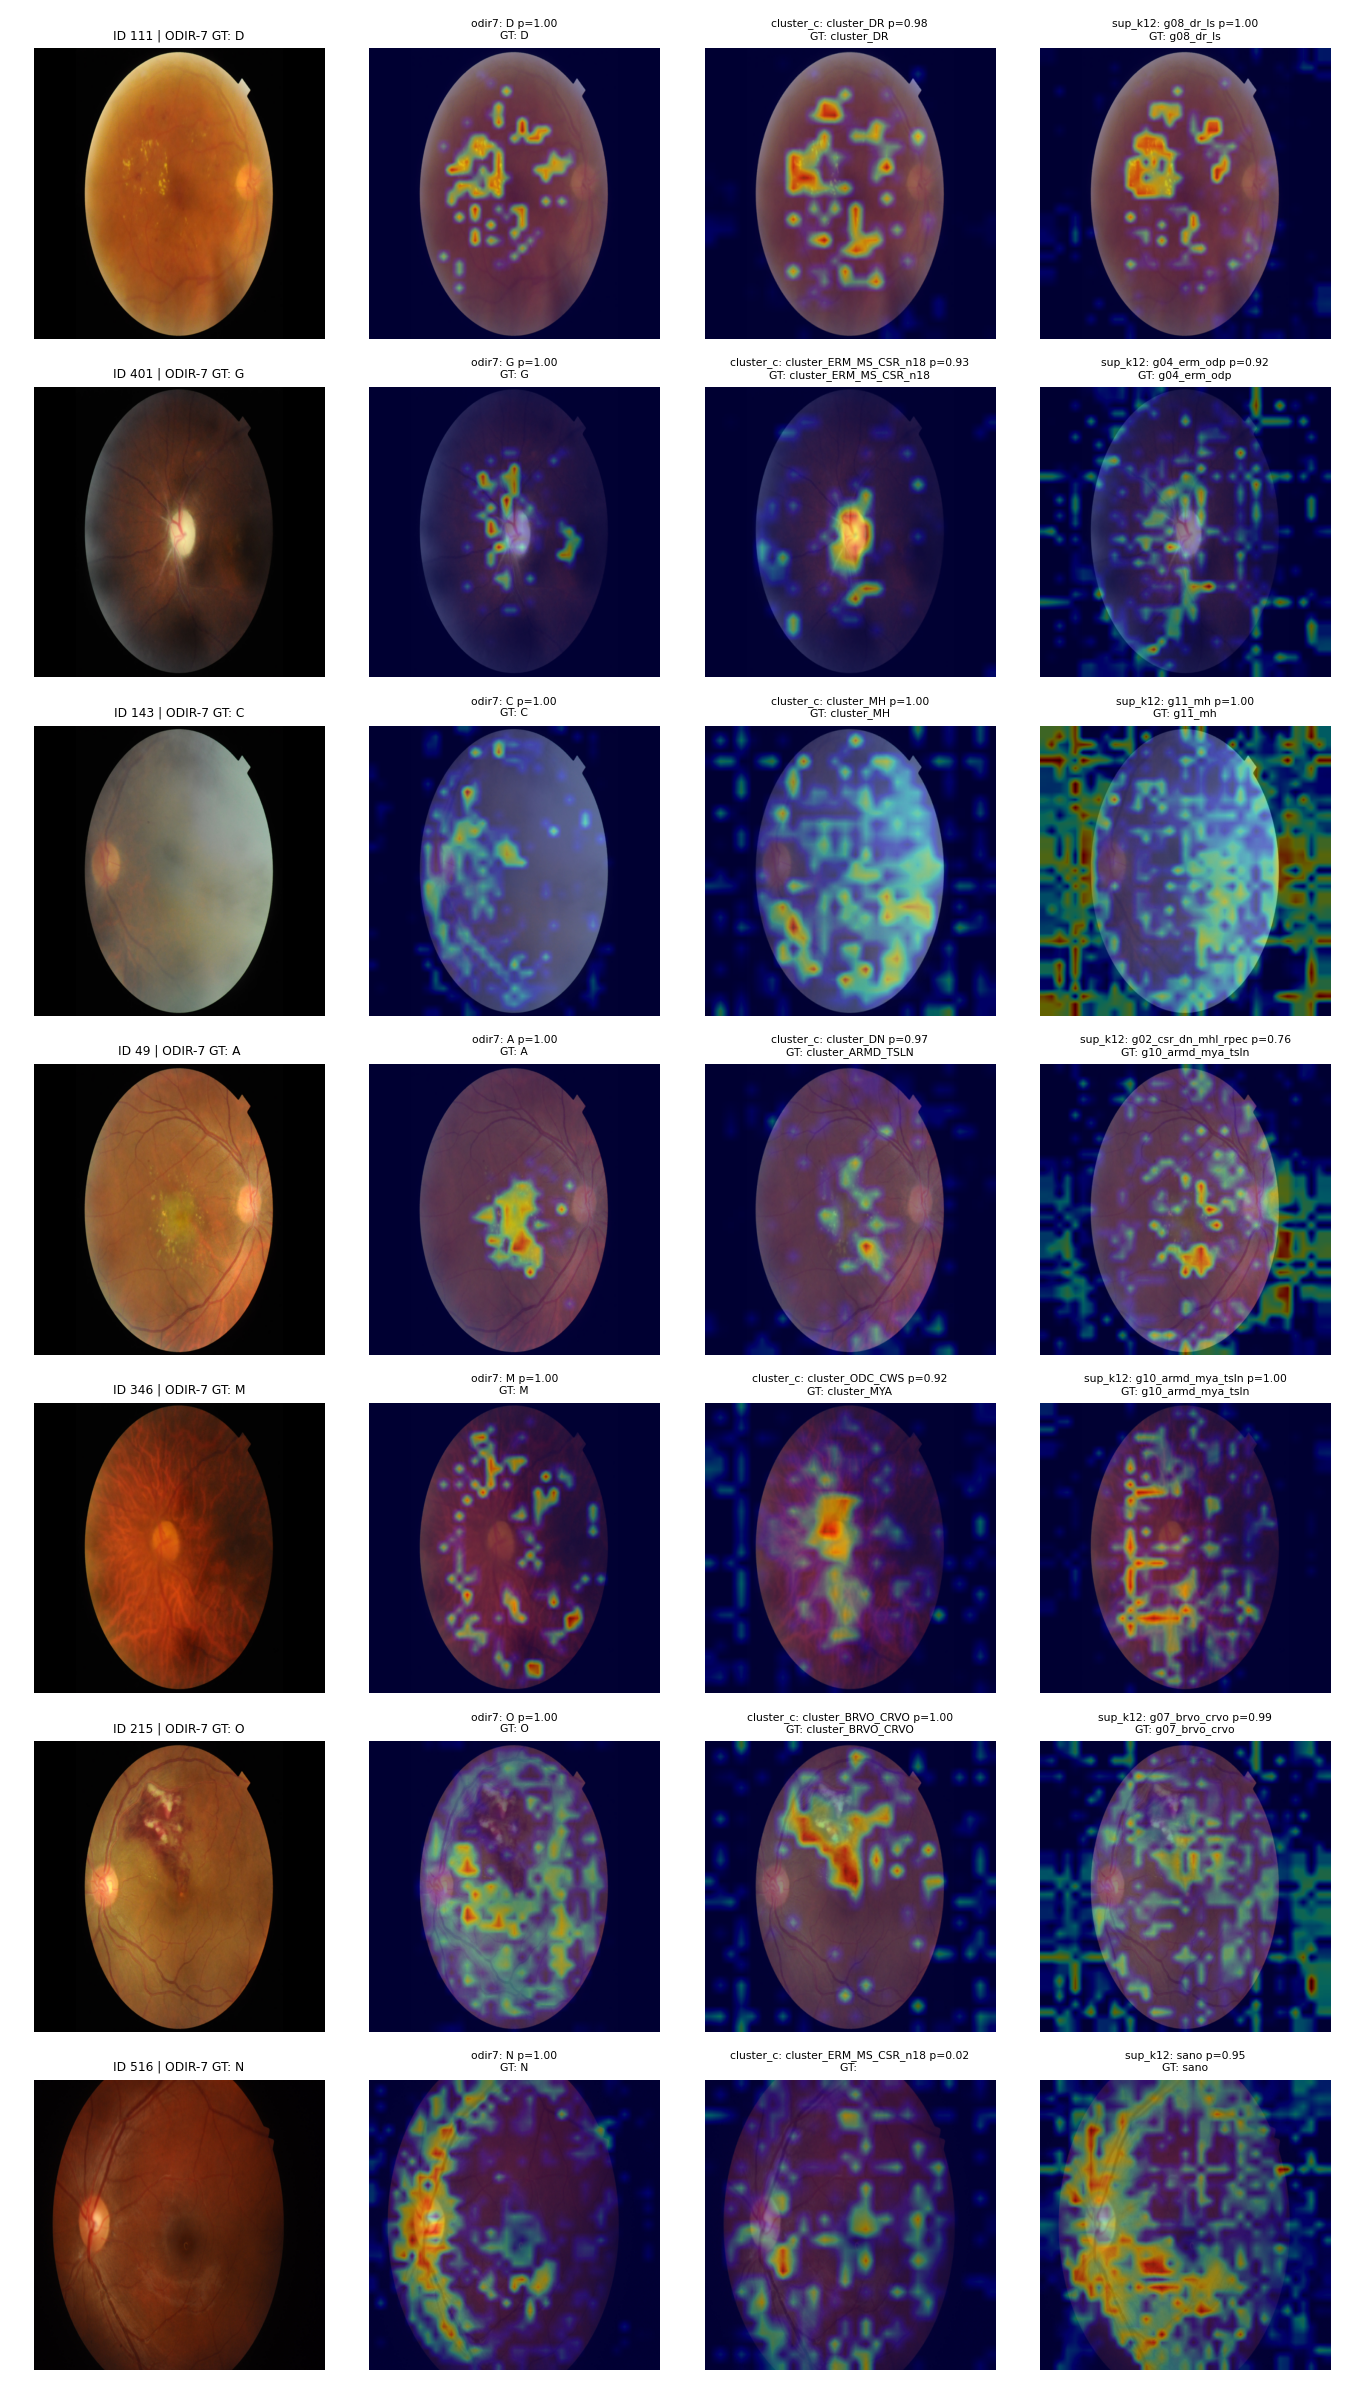
\includegraphics[width=\textwidth]{figures/gradcam_comparison.png}
\caption{Grad-CAM on seven test images (columns: one per ODIR-7 label) for the ODIR-7, Cluster-C and Sup-K12 models (rows). Qualitative only; the maps are not lesion segmentations.}
\label{fig:gradcam}
\end{figure*}

\section{Discussion}
\textbf{Taxonomy matters more than architecture.}
The same images and similar backbones give macro $F_2$ values of 0.81--0.84 on ODIR-7, 0.77 on Cluster-C and 0.63--0.69 on Sup-K12.
The difference comes mainly from the number of labels and from how many labels have few positives: Sup-K12 keeps rare groups (4--14 test positives) that dominate the macro average.
Numbers from different taxonomies, including the macro AUROC of 0.904 of our earlier ten-label study, are therefore not directly comparable, and any claim of improvement should be made within one taxonomy.

\textbf{Small ensembles are a robust gain.}
Two- or three-member ensembles never hurt and gave significant gains in AUROC and mAP in all taxonomies, and in $F_2$ in two of three.
On Sup-K12 the ensemble also protects against an unlucky single-model choice: the validation-selected single model ranks only ninth on test, while the ensemble is close to the best single model on test.

\textbf{Retinal initialisation.}
Contrary to our expectation, RETFound-DINOv2 initialisation did not improve over DINOv2 under the same recipe. Fundus-initialised models are, however, useful ensemble members (they appear in the selected ODIR-7 and Cluster-C ensembles), which suggests that their errors are partly decorrelated from those of the DINOv2 models.

\textbf{Resolution, head and backbone.}
$518$\,px helped only on Cluster-C, at roughly twice the cost of $392$\,px. The residual attention head helped on ODIR-7 only. Both effects are about the size of the seed variation, so they should be confirmed over several seeds.
The BFPC-style ResNet-50 baselines were consistently below the ViTs. The very high scores reported for BFPC-Net on ODIR~\cite{li2022bfpc} are not comparable with ours, because the dataset, the labels (binocular, patient-level) and the metrics differ.

\textbf{Recall-priority operating points.}
The F2-opt thresholds give high recall (0.91 on ODIR-7) at a macro precision of about 0.6, which suits screening, where a missed disease is costlier than a false alarm. The R$\geq$0.8 rule trades recall for precision more predictably on the larger taxonomies, but on Sup-K12 it misses its target on test.

\textbf{Limitations.}
(i) \emph{Missing checkpoints.} Several models, including all members of the Sup-K12 ensemble and the Cluster-C ViT-RA 518, are available only as stored predictions, not as weights. Their metrics are fully reproducible from the predictions, but Grad-CAM had to use proxies and these models cannot be deployed.
(ii) \emph{Possible leakage through pre-training.} The FLAIR encoder used for one BFPC baseline was pre-trained on a collection of public fundus datasets that may include RFMiD images; this was not verified. Whether RETFound's pre-training data include RFMiD was not verified either. Any such overlap would make the fundus-initialised results optimistic.
(iii) \emph{No external validation.} All results come from a single source dataset of limited size without patient identifiers, so patient overlap across splits cannot be excluded and generalisation to other cameras and populations is untested.
(iv) \emph{Shortcut risk.} The border and background activations of the Sup-K12 proxy suggest a possible reliance on image borders or the acquisition field, which we did not test (e.g.\ with masking).
(v) \emph{Selection and variance.} Selection uses validation only, but validation also serves for early stopping and thresholds. Most configurations have a single seed, and the seed spread (up to 0.068 in $F_2$) is comparable to many configuration differences.
(vi) \emph{Proxy labels.} ODIR-7 ``C'' and ``G'' are proxies (media opacity, optic-disc findings), not cataract and glaucoma diagnoses, and the clustered taxonomies have no clinical definition.
(vii) \emph{Grad-CAM} is qualitative, on seven images, and RFMiD has no lesion masks.
(viii) This is a research prototype, not a medical device and not a substitute for a physician.

\section{Conclusion and Future Work}
Across three RFMiD label taxonomies, a partially fine-tuned DINOv2 ViT-L/14 with a residual attention token head and validation-fitted, recall-priority thresholds is the strongest single family. Small validation-selected ensembles reach test macro $F_2$ values of 0.835 (ODIR-7), 0.775 (Cluster-C) and 0.687 (Sup-K12), with macro AUROCs of 0.937--0.954.
Ensembling is the most reliable improvement. Retinal foundation initialisation, higher resolution and the attention head give small or taxonomy-dependent effects that are of the order of the seed variance.
Grad-CAM maps are plausible on ODIR-7 but show possible border shortcuts for the class-token Sup-K12 model.

Future work includes several seeds per configuration, an untouched hold-out set, external validation on other datasets (e.g.\ ODIR), checking the pre-training corpora of the fundus encoders for RFMiD overlap, border-masking tests for shortcuts, calibration, and a quantitative evaluation of the explanations.

\section*{Reproducibility}
Per-model predictions, the unified bootstrap comparison (\texttt{results/final\_comparison\_20261030}) and the figure/table script for this paper (\texttt{paper/figures\_v3\_20261102}) are in the project repository.
% TODO: add public repository URL and licence, and the data-use statement for RFMiD.

\bibliographystyle{IEEEtran}
\bibliography{references}

\end{document}
